\documentclass[10pt,conference]{IEEEtran}
\IEEEoverridecommandlockouts

\usepackage[utf8]{inputenc}
\usepackage[T1]{fontenc}
\usepackage[brazilian]{babel}
\usepackage{cite}
\usepackage{amsmath,amssymb,amsfonts}
\usepackage{graphicx}
\usepackage{textcomp}
\usepackage{xcolor}
\usepackage{booktabs}
\usepackage{url}
\usepackage{balance}

\begin{document}

\title{Quem de Fato Colabora nos Repositórios Web3?\\
Evidência Preliminar sobre Core e Occasional Contributors}

\author{\IEEEauthorblockN{Pamella Soares}
\IEEEauthorblockA{Universidade Estadual do Ceará (UECE)\\
Fortaleza, Brasil\\
pamella.soares@aluno.uece.br}
}

\maketitle

\begin{abstract}
Narrativas sobre open source Web3 frequentemente pressupõem colaboração ampla. Neste \emph{work-in-progress}, provocamos essa premissa: \textbf{quem de fato concentra a colaboração observável} em repositórios \emph{provider}? Usando o Web3BlockSet~\cite{soares2026web3blockset} (somente providers; 2018--2025), rotulamos \emph{core} como o top 10\% de autores por Issues/PRs abertos em cada repositório e contrastamos com \emph{occasional contributors}. Em 316 repositórios ($\approx$360k documentos; 59k autores), o core abre \textbf{69\%} dos documentos; aparece em \textbf{59\%} das threads iniciadas por occasionals; e o Gini mediano de autoria é \textbf{0,55}. Ano a ano, a concentração na abertura permanece alta, enquanto a taxa de aparição do core em threads da periferia \emph{cai} (0,69$\rightarrow$0,36). Escopo deliberadamente limitado---sem topic modeling nem SPACE/BcDEx~\cite{soares2025bcdex}.
\end{abstract}

\begin{IEEEkeywords}
Mining Software Repositories, Web3, colaboração, core developers, work-in-progress
\end{IEEEkeywords}

\section{Introdução e Provocação}

Em ecossistemas Web3, é comum falar em ``comunidade de desenvolvedores''. Porém, a atividade observável em OSS costuma ser desigual entre núcleo e periferia~\cite{das2022blockchain,joblin2017classifying}. A provocação deste short é:

\begin{quote}
\emph{Se $\approx$10\% dos autores abrem a maior parte dos Issues/PRs---e ainda assim o núcleo participa de boa parte das threads da periferia---então métricas e políticas que tratam a comunidade como massa homogênea podem estar otimizando um mito.}
\end{quote}

Esta nota não fecha o debate sobre saúde de comunidades Web3. Nos termos do MSR para \emph{work-in-progress}, seu papel é apresentar uma ideia controversa/interessante com evidência preliminar suficiente para discussão---não a avaliação completa de um full paper.

\textbf{RQ:} Como se diferenciam \emph{core} e \emph{occasional contributors} na colaboração observável (abertura e participação em threads) dos repositórios provider do Web3BlockSet (2018--2025)?

\paragraph{Por que isto é WIP.}
Não estimamos causalidade de retenção, não fechamos validação de afiliação organizacional em escala e \textbf{não} reanalizamos ``dores''/DEx em BaaS~\cite{soares2025bcdex}. A contribuição é reposicionar o olhar: de \emph{o que} se discute para \emph{quem} sustenta a colaboração observável.

\section{Trabalho Relacionado (posicionamento)}

A distinção core/periferia é clássica em engenharia de software aberta. Joblin et al.~\cite{joblin2017classifying} mostram que métricas de contagem e de rede classificam desenvolvedores em núcleo e periferia com implicações para coordenação. Em blockchain, Das et al.~\cite{das2022blockchain} caracterizam colaboração em repositórios GitHub, enquanto tipologias de issues~\cite{opu2025issuetypes} e a agenda BOSE~\cite{porru2017bose} enfatizam especificidades do domínio. O Web3BlockSet~\cite{soares2026web3blockset} habilita análises em escala com categorias de stack validadas. Já estudos de BcDEx em BaaS~\cite{soares2025bcdex} aprofundam \emph{o que} se discute e dimensões de produtividade/experiência.

Este WIP ocupa um espaço ortogonal: não pergunta quais tópicos doem, e sim \textbf{quão concentrada} é a colaboração observável e como core e occasionals se relacionam em threads. Usamos métricas simples e replicáveis (top 10\%, Gini/HHI, participação do core em threads da periferia), explicitamente evitando overlap com topic modeling e SPACE.

\section{Dados e Método (limitado)}

\subsection{Corpus}
Issues/PRs com \texttt{data\_source=provider} e \texttt{repository\_category} validada no Web3BlockSet~\cite{soares2026web3blockset}, anos 2018--2025. Após filtros ($\geq$30 documentos/repo), permanecem 316 repositórios, $\approx$360\,183 documentos e 59\,141 autores. Campos centrais: \texttt{author}, \texttt{comment\_authors} (separados por `;`), repositório e categoria.

\subsection{Definição operacional de papéis}
Em cada repositório, ordenamos autores pelo número de Issues/PRs \emph{abertos} e definimos:
\begin{itemize}
\item \textbf{core:} top 10\% dos autores (pelo menos um);
\item \textbf{occasional:} demais autores.
\end{itemize}
Essa definição torna o share de documentos um \emph{resultado} (não uma tautologia do tipo ``core = quem faz 80\%''). A categoria do stack entra apenas como estratificação secundária.

\subsection{Métricas}
(1)~Gini e HHI da distribuição de autoria por repositório; (2)~share global/anual de documentos abertos pelo core; (3)~taxa em que algum autor core aparece em \texttt{comment\_authors} quando o opener é occasional; (4)~número médio de comentadores únicos por thread; (5)~Gini mediano por categoria validada.

\subsection{Validação manual}
Amostra cega estratificada por categoria$\times$papel automático (\texttt{data/manual\_review/}; $n{=}445$) pede a revisores inferir o papel real (\texttt{core\_maintainer}, \texttt{regular}, \texttt{occasional}, \texttt{bot\_or\_automation}, \texttt{unsure}) e afiliação aparente à organização, sem ver o rótulo automático. Protocolo em \texttt{PROTOCOL\_MANUAL\_REVIEW.md}. Neste WIP descrevemos o desenho; $\kappa$ e precisão entram após dupla anotação.

\section{Evidência Preliminar}

\begin{figure}[t]
\centering
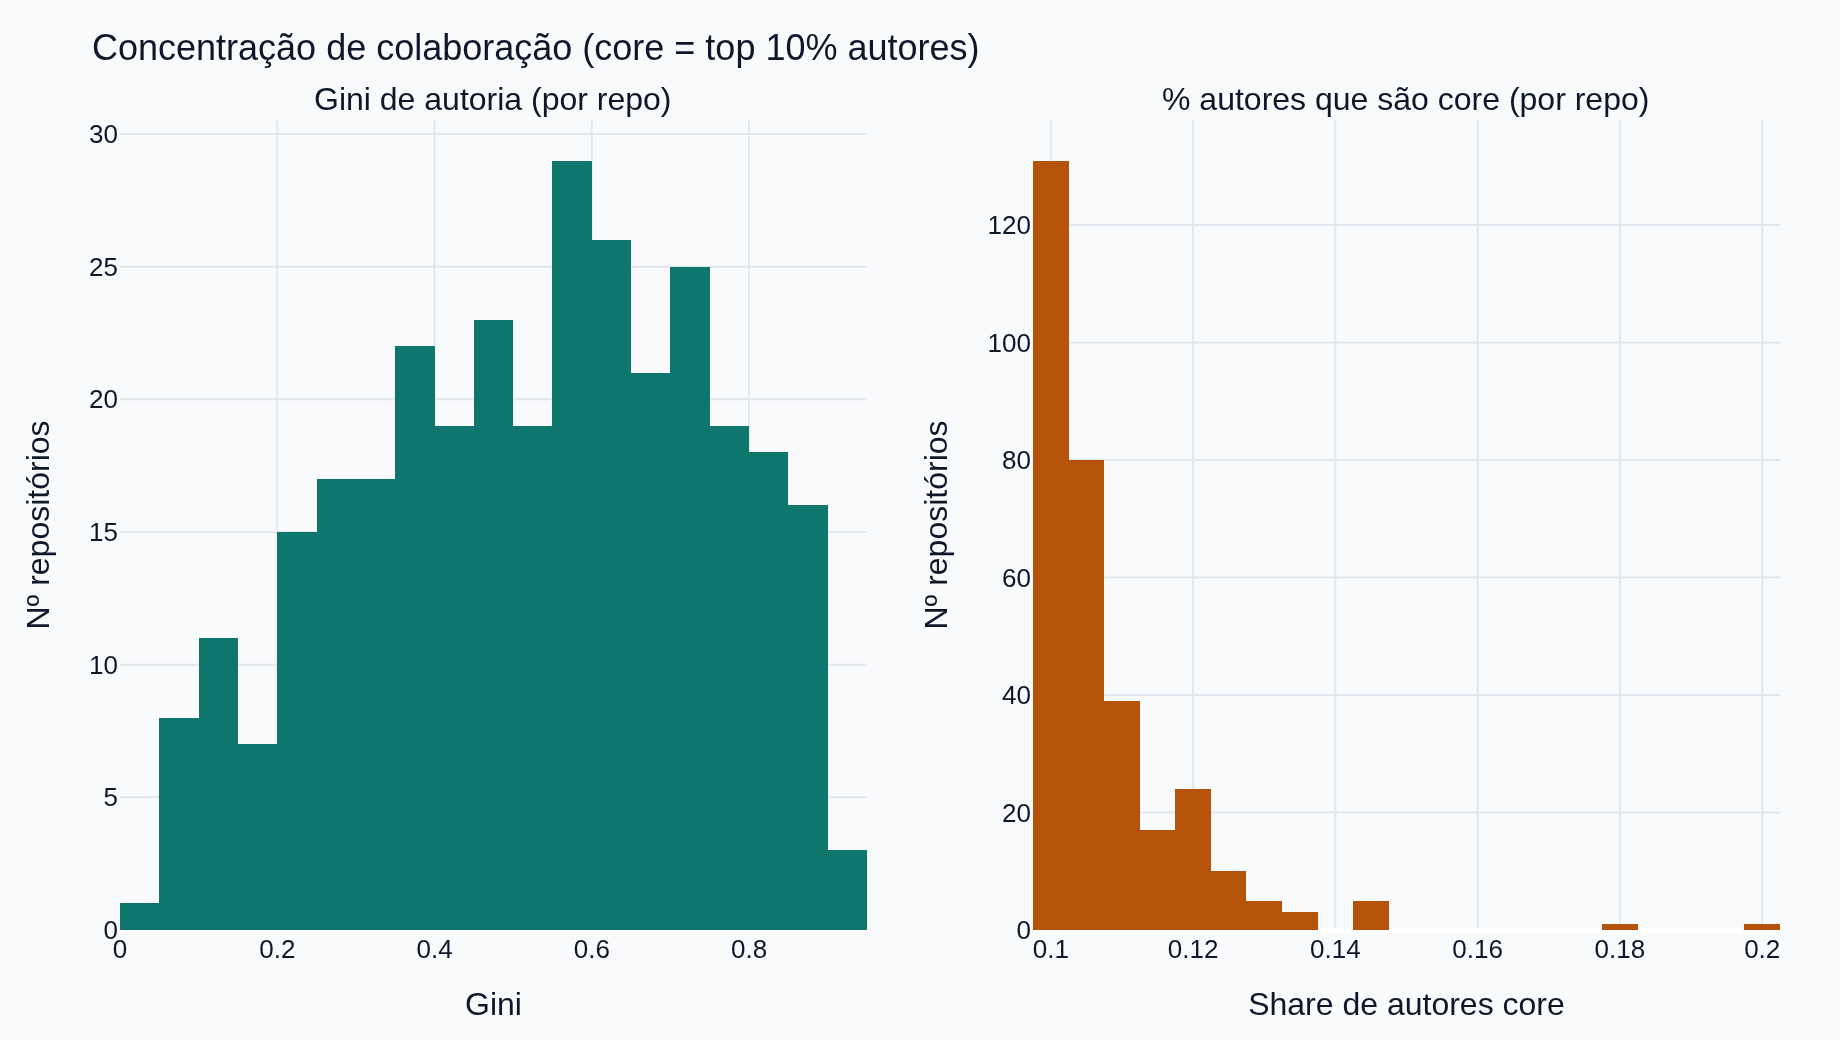
\includegraphics[width=\columnwidth]{figures/fig1_concentration_dist.png}
\caption{Distribuição, entre repositórios, do Gini de autoria e da fração de autores no core (top 10\%).}
\label{fig:dist}
\end{figure}

\begin{figure}[t]
\centering
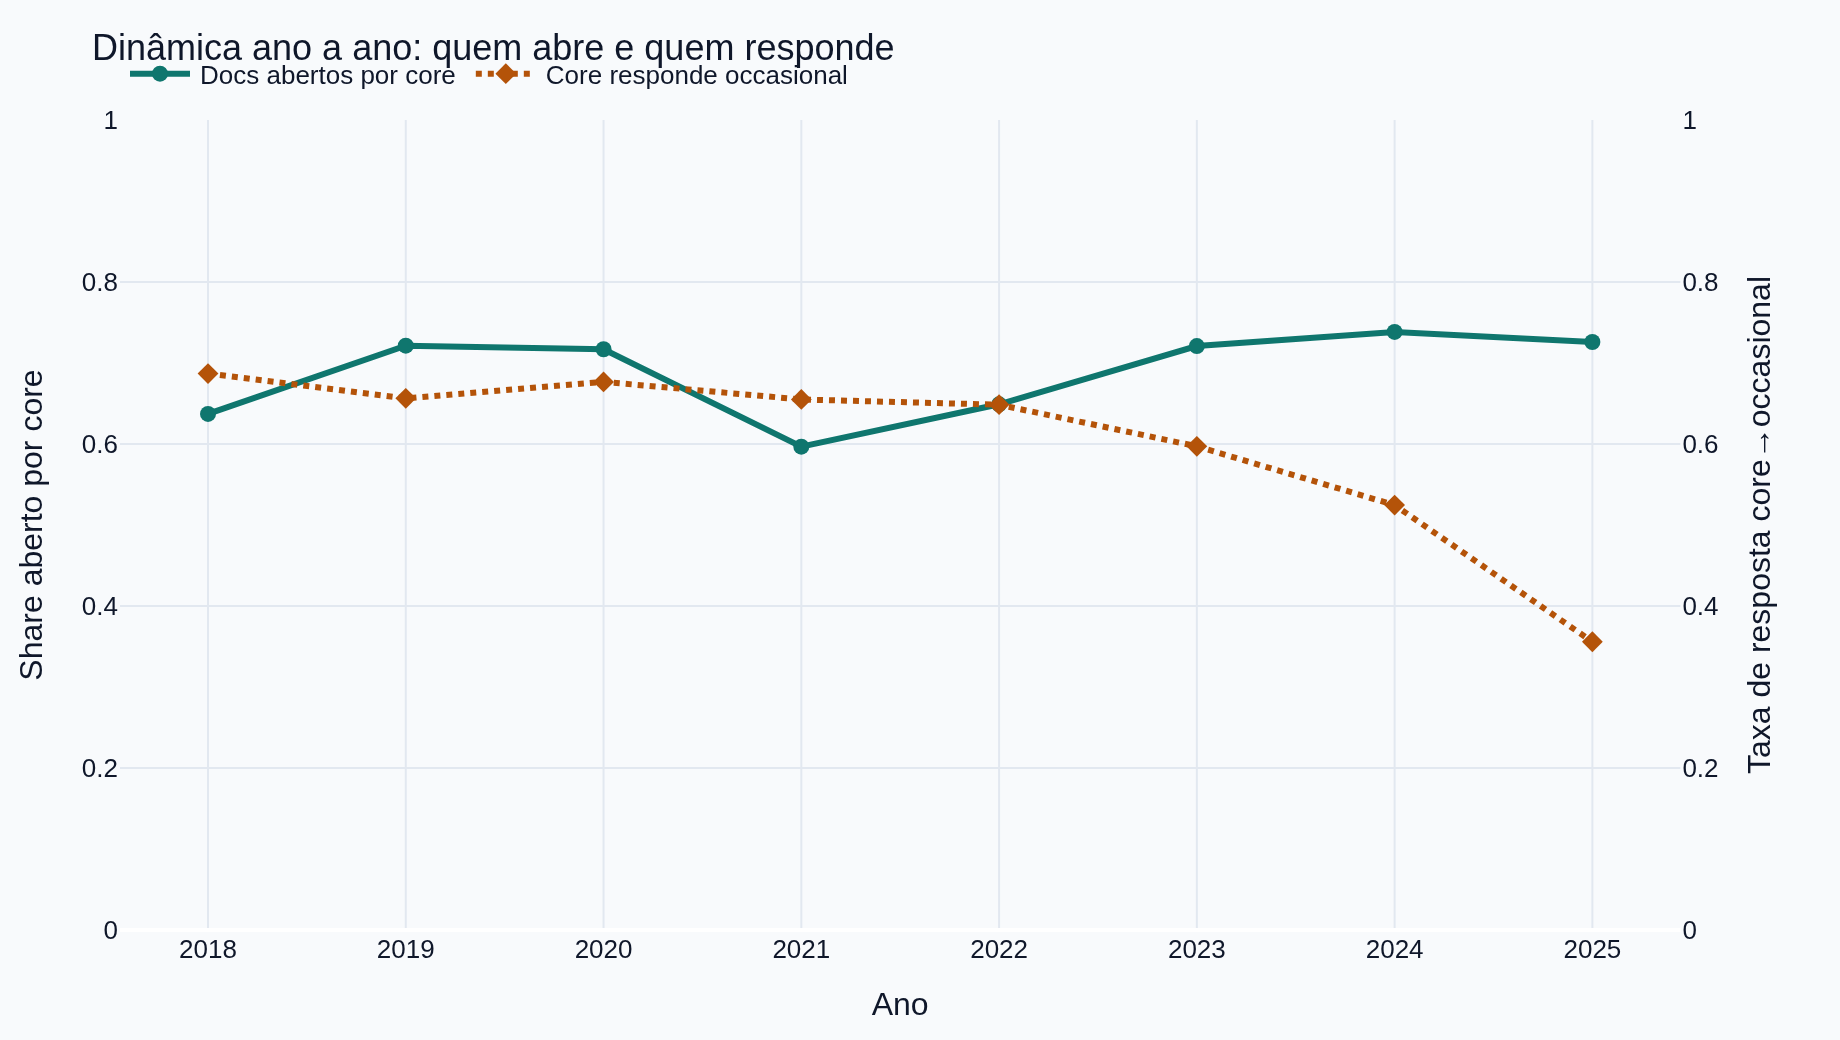
\includegraphics[width=\columnwidth]{figures/fig2_yearly_roles.png}
\caption{Ano a ano: share de documentos abertos pelo core e taxa de aparição do core em threads iniciadas por occasionals.}
\label{fig:yearly}
\end{figure}

\begin{figure}[t]
\centering
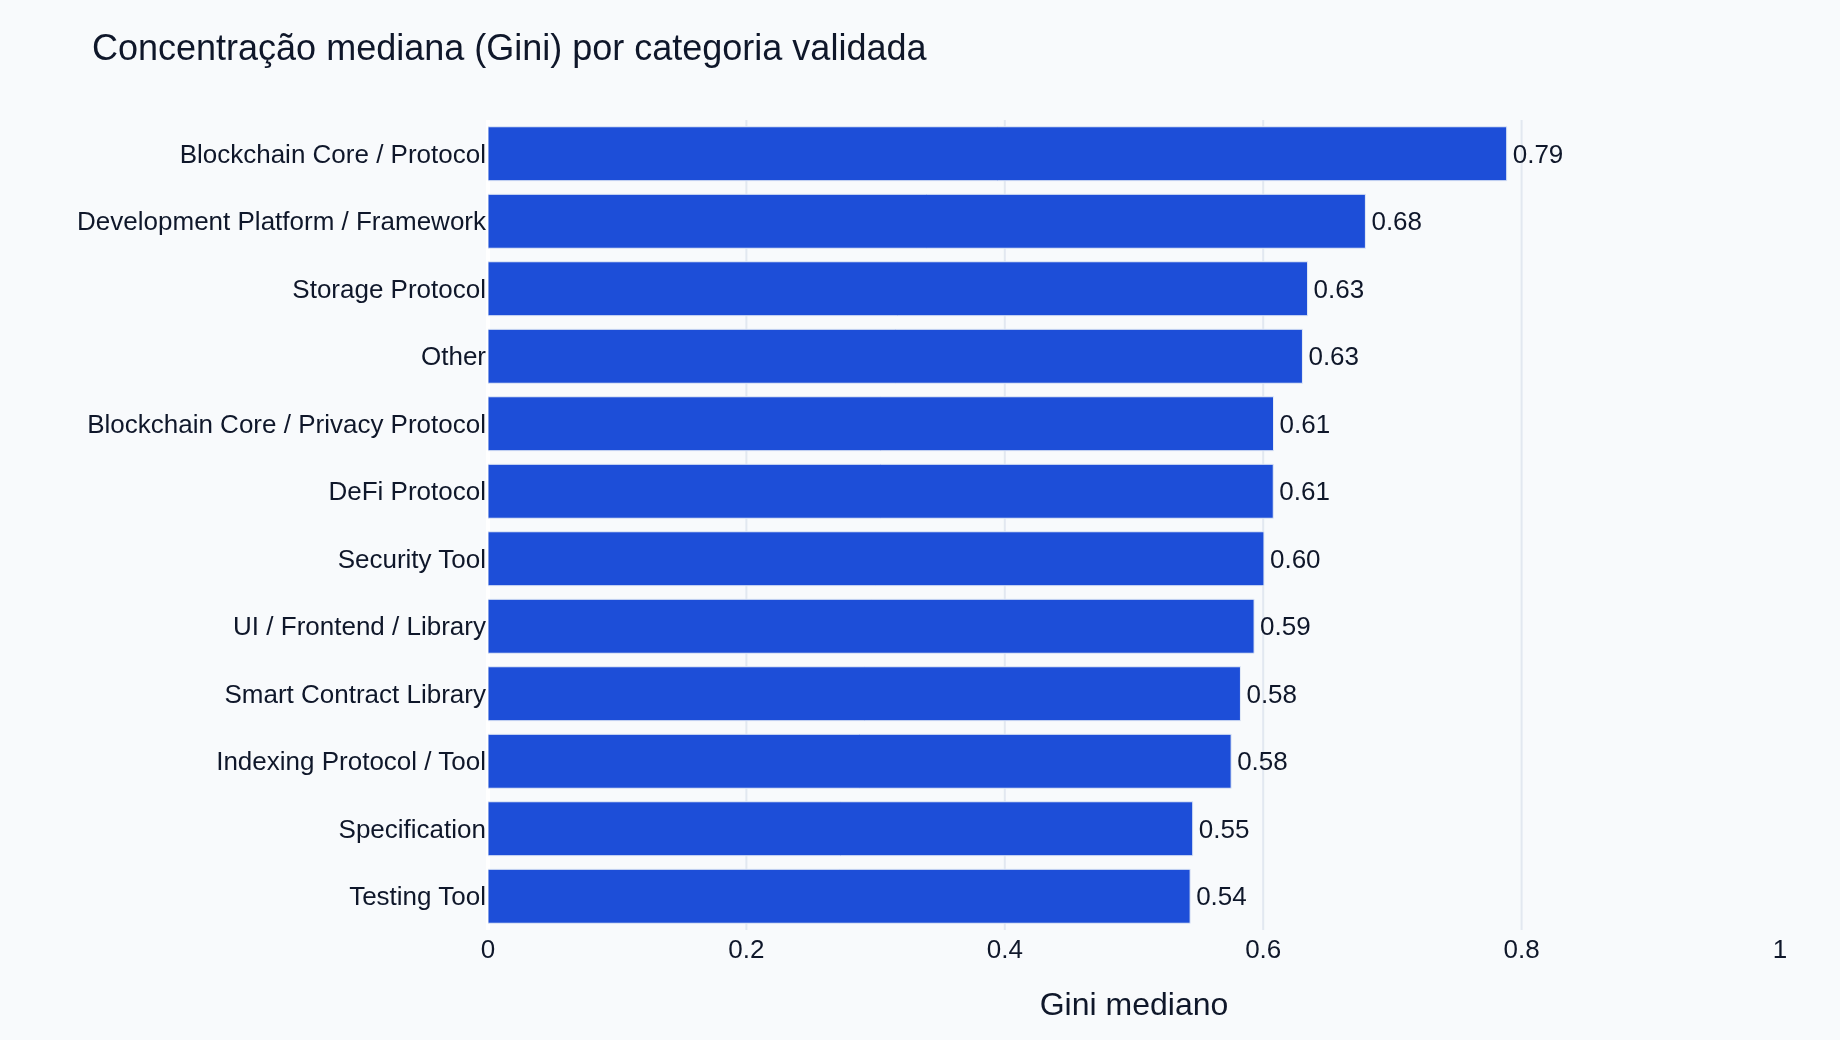
\includegraphics[width=\columnwidth]{figures/fig3_gini_by_category.png}
\caption{Gini mediano por categoria validada (repositórios com atividade suficiente).}
\label{fig:cat}
\end{figure}

\begin{figure}[t]
\centering
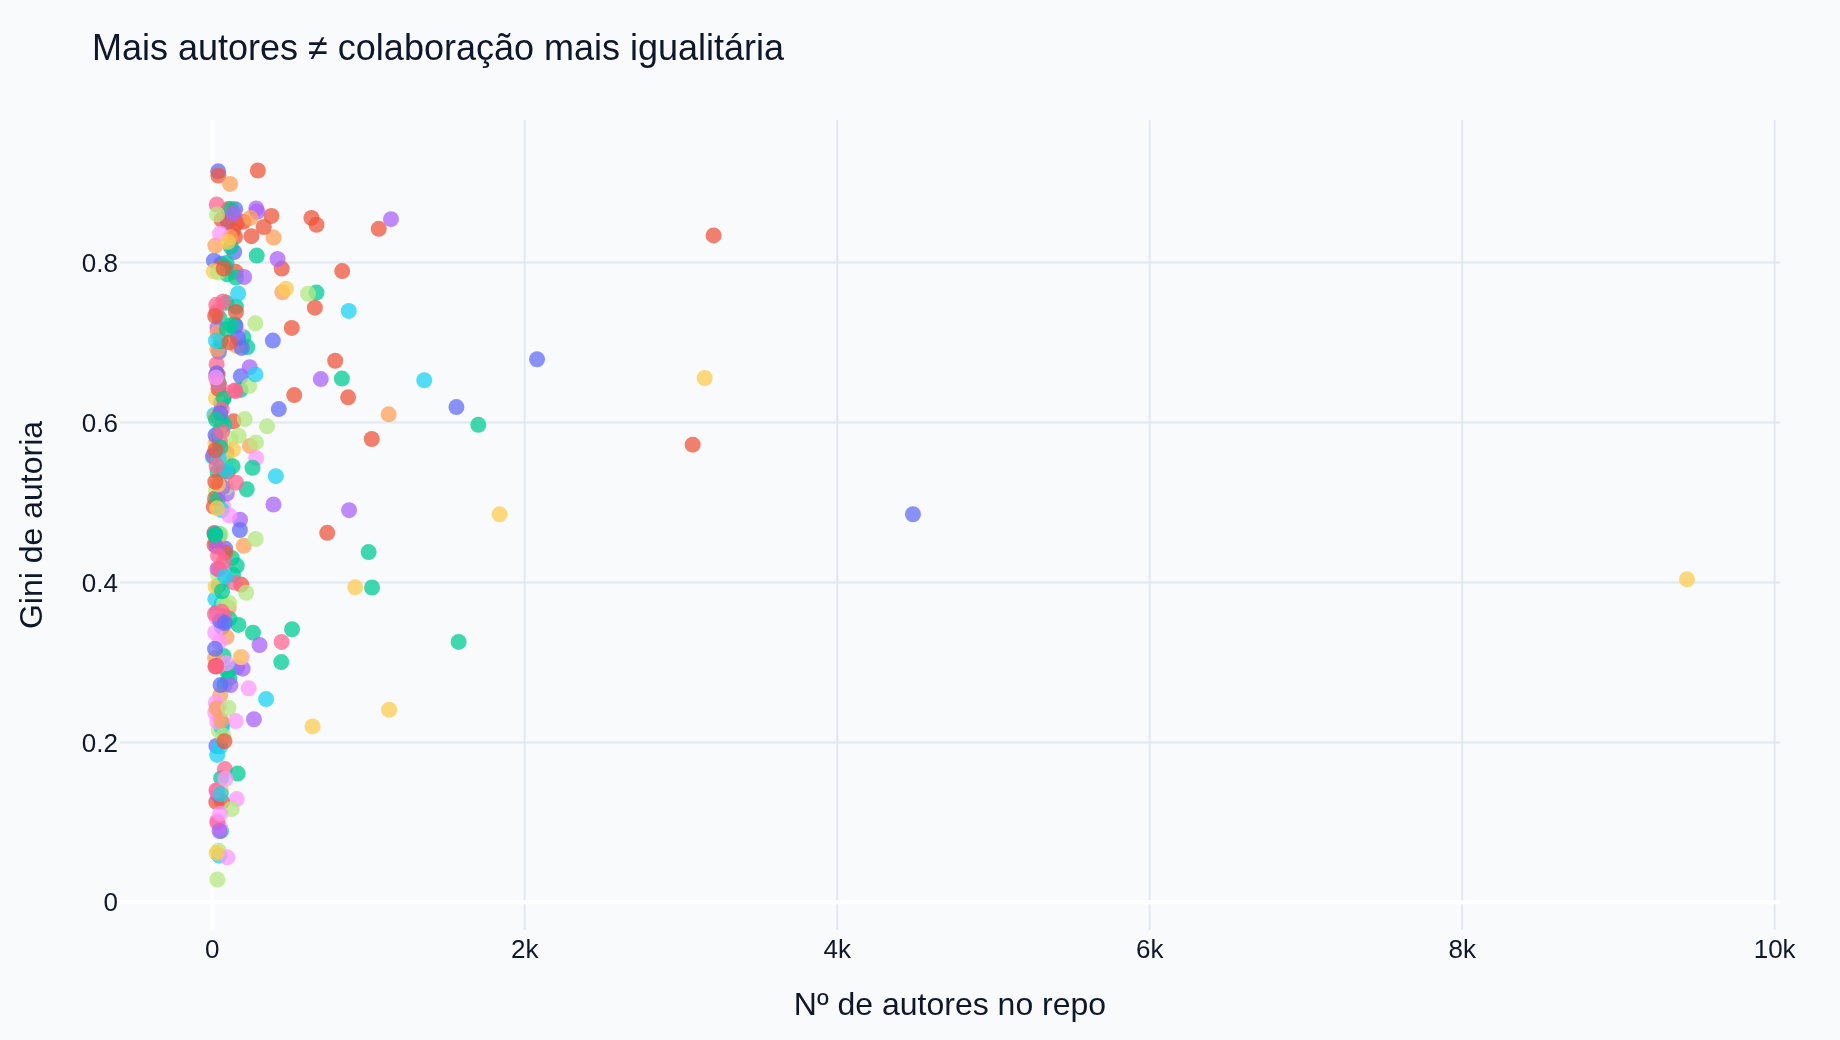
\includegraphics[width=\columnwidth]{figures/fig4_authors_vs_gini.png}
\caption{Número de autores versus Gini: ter muitos participantes não implica colaboração igualitária.}
\label{fig:scatter}
\end{figure}

\paragraph{Achado 1---Concentração na abertura.}
O top 10\% de autores abre \textbf{69,1\%} dos documentos no corpus filtrado. O Gini mediano por repositório é \textbf{0,55}; a mediana é de $\approx$8--9 autores core em $\approx$80 autores/repo (Figura~\ref{fig:dist}). Isso sustenta a provocação de assimetria: a ``comunidade'' listável é maior do que o conjunto que de fato impulsiona a maior parte da atividade observável.

\paragraph{Achado 2---O core ainda atravessa a periferia.}
Em \textbf{59,0\%} das threads abertas por occasionals, algum autor core aparece em \texttt{comment\_authors}. Ou seja, mesmo quando a periferia inicia a conversa, o núcleo frequentemente permanece na thread---padrão compatível com suporte, revisão ou triagem centralizada.

\paragraph{Achado 3---Dinâmica temporal (miolo anual).}
Entre 2018 e 2025 (Figura~\ref{fig:yearly} e Tabela~\ref{tab:yearly}), a share de documentos abertos pelo core permanece alta ($\approx$0,64--0,74). Em contraste, a taxa de aparição do core em threads da periferia \textbf{declina} de 0,69 (2018) para 0,36 (2025). O número médio de comentadores únicos por thread também cai (1,63$\rightarrow$0,64). Essa combinação é thought-provoking: não vemos ``democratização'' da abertura; vemos possível \emph{afastamento relativo} do núcleo nas conversas da periferia (hipótese a testar---pode refletir escala, automação, ou mudança de canais para Discord/fora do GitHub).

\begin{table}[t]
\caption{Métricas anuais de colaboração (providers).}
\label{tab:yearly}
\centering
\scriptsize
\begin{tabular}{@{}rrrrr@{}}
\toprule
Ano & Docs & Core abre & Core em occ. & Gini med. \\
\midrule
2018 & 24\,699 & 0,64 & 0,69 & 0,46 \\
2019 & 27\,619 & 0,72 & 0,66 & 0,47 \\
2020 & 33\,918 & 0,72 & 0,68 & 0,49 \\
2021 & 48\,057 & 0,60 & 0,65 & 0,43 \\
2022 & 53\,755 & 0,65 & 0,65 & 0,42 \\
2023 & 57\,330 & 0,72 & 0,60 & 0,49 \\
2024 & 57\,482 & 0,74 & 0,52 & 0,49 \\
2025 & 57\,323 & 0,73 & 0,36 & 0,50 \\
\bottomrule
\end{tabular}
\end{table}

\paragraph{Achado 4---Heterogeneidade por categoria.}
O Gini mediano varia entre camadas do stack (Figura~\ref{fig:cat}). Portanto, generalizações ``Web3-wide'' sobre colaboração podem falhar se ignorarem o tipo de repositório. A Figura~\ref{fig:scatter} reforça que \emph{mais autores} não implicam automaticamente menor desigualdade.

\paragraph{Achado 5---Escala não equaliza.}
Repositórios com dezenas ou centenas de autores ainda podem exibir Gini elevado. Em outras palavras, ``muitos nomes'' no histórico de Issues/PRs é evidência fraca de colaboração distribuída. Para o WIP, isso importa porque dashboards baseados apenas em contribuidores únicos tendem a superestimar amplitude comunitária.

\subsection{Síntese da provocação}
Combinando os achados: (i)~poucos abrem a maior parte; (ii)~o núcleo ainda aparece em muitas threads da periferia; (iii)~essa ponte enfraquece no tempo; (iv)~o grau de concentração depende da camada. A leitura controversa---ainda hipotética---é que parte do discurso de ``comunidade Web3'' descreve uma periferia larga acoplada a um núcleo pequeno, e que o acoplamento observável no GitHub pode estar diminuindo sem que a desigualdade na abertura desapareça.

\section{Impacto, atenções e remediações}

\subsection{Impacto no ecossistema Web3}
\begin{itemize}
\item \textbf{Pesquisa:} agregar todos os autores como ``comunidade'' mistura regimes core/periferia e pode inflar percepções de engajamento.
\item \textbf{Foundations/plataformas:} bus factor---poucos abrem a maior parte da atividade observável; sucessão e distribuição de carga importam.
\item \textbf{Onboarding:} volume de nomes em Issues $\neq$ rede densa; newcomers provavelmente interagem com um núcleo pequeno.
\item \textbf{Governança e suporte:} se a participação do core nas threads da periferia cai ao longo do tempo, há risco de fila não atendida e churn de contribuidores ocasionais---mesmo com alta concentração na abertura.
\item \textbf{Métricas de saúde OSS:} dashboards que só contam contribuidores únicos podem pintar um quadro otimista demais.
\end{itemize}

\subsection{Atenções (ameaças ao overclaim)}
\begin{itemize}
\item Top-10\% é proxy de papel, não membership GitHub nem ``maintainer'' oficial.
\item Bots residuais podem inflar ou distorcer caudas.
\item \texttt{comment\_authors} pode estar incompleto; ausência de core na lista $\neq$ ausência real de resposta.
\item Queda da taxa de participação pode refletir crescimento do volume, migração para outros canais, ou mudança de práticas---não necessariamente desengajamento deliberado.
\item Resultados são para providers; não generalizamos para adopters community.
\end{itemize}

\subsection{Remediações recomendadas}
\begin{itemize}
\item Sempre reportar métricas separadas para core vs periferia.
\item Monitorar bus factor e tempo/participação em threads abertas por occasionals.
\item Validar papéis (amostra manual + afiliação organizacional via API).
\item Em estudos futuros, ligar papéis a retenção (ponte natural para a RQ3b do Web3BlockSet) e a redes de co-comentário.
\end{itemize}

\section{Ameaças à Validade}

\paragraph{Construto.}
Abertura de Issues/PRs captura iniciativa observável, não horas de trabalho nem qualidade. Participação em \texttt{comment\_authors} é proxy grosseiro de ``resposta''.

\paragraph{Interna.}
A escolha do limiar 10\% é convencional; sensibilidades (5\%/15\%) ficam para o full paper. Repositórios pequenos foram excluídos ($<$30 docs), o que pode enviesar para projetos mais ativos.

\paragraph{Externa.}
Cobertura do Web3BlockSet e foco em providers limitam generalização. Ecossistemas fora de GitHub não são observados.

\paragraph{Confiabilidade.}
A amostra cega ($n{=}445$) ainda precisa de dupla anotação; até lá, a heurística deve ser lida como operacionalização transparente, não como ground truth.

\section{Próximos Passos}
\begin{enumerate}
\item fechar dupla anotação cega e reportar precisão/$\kappa$ da heurística top-10\%;
\item segundo critério de core via afiliação organizacional (GitHub org members);
\item redes de co-comentário e centralidade ao longo do tempo;
\item analisar se a queda da participação do core persiste após normalizar por volume;
\item ponte com retenção de contribuidores (RQ3b);
\item full paper com hipóteses pré-registradas e análises de sensibilidade.
\end{enumerate}

\section{Implicações para o desenho de estudos futuros}

Se os padrões se confirmarem sob validação manual e sensibilidades de limiar, sugerimos três práticas mínimas em estudos MSR sobre Web3: (1)~\textbf{sempre} separar core e periferia ao reportar atividade; (2)~acompanhar não só volume de contribuidores, mas \emph{quem responde a quem}; (3)~estratificar por categoria de repositório quando a pergunta for sobre o ecossistema como um todo. Essas práticas são baratas, alinhadas a open science, e reduzem o risco de conclusões infladas sobre ``engajamento comunitário''.

\section{Conclusão}

Este WIP desloca o foco de ``o que dói nos desenvolvedores Web3'' para \textbf{quem sustenta a colaboração observável}. Evidência preliminar em providers: poucas pessoas abrem a maior parte da atividade; o núcleo ainda atravessa muitas threads da periferia; e essa ponte parece enfraquecer no tempo. A provocação---ainda em formação---é que pesquisas e práticas não deveriam tratar a comunidade Web3 como massa homogênea. O valor do short está em tornar essa tensão discutível com dados, figuras e um protocolo de validação já preparado---não em encerrar o caso.

\section*{Disponibilidade de Dados}
Artefatos (scripts, tabelas, figuras, protocolo e amostra cega) estão em \texttt{2027\_short\_paper\_3a}. O dataset-base é o Web3BlockSet~\cite{soares2026web3blockset}. Para submissão double-anonymous, o pacote será depositado de forma anonimizada.

\bibliographystyle{IEEEtran}
\bibliography{references}

\end{document}
